Consider the well-known circles derived from a reference triangle and their radii, listed on Table~\ref{tab:four-more}.

\begin{table}
\begin{tabular}{|l|l|l|l|}
\hline
Circle & Description (see \cite{mw}) & Center & Radius\\
\hline
Anticompl. & Circumc. of Anticompl. & $X_{4}$ & $2R$\\
Bevan & Circumc. of Excentral & $X_{40}$ & $2R$ \\
Spieker & Incircle of Medial & $X_{10}$ & $r/2$ \\
Mandart & Circumc. of Extouch & $X_{1158}$ & see \eqref{eqn:mandart-radius} \\
\hline
\end{tabular}
\caption{Definition of certain circles for which under certain families the power of the center is also invariant. $R,r$ denote circumradius and inradius.}
\label{tab:four-more}
\end{table}

Let $s$ denote the semiperimeter. The radius of the Mandart circle is given by \cite[Mandart Circle]{mw}:

\begin{equation}
R_m=\frac{s}{s_1 s_2 s_3}\sqrt{(4R^2-s_2 s_3)(4 R^2-s_3 s_1)(4R^2-s_1 s_2)}
\label{eqn:mandart-radius}
\end{equation}

Referring to Figure~\ref{fig:four-more}, for selected families, the power of the center is also invariant.

\begin{proposition}
Over the homothetic family, the power of the center with respect to the anticomplementary circle is given by:

\[ \P_{4,act}= {-(4/9)\sum{s_i}^2}\]
\end{proposition}

\begin{proposition}
Over the confocal family, the power of the center with respect to the Bevan, Spieker, and Mandart circles are given by:

\begin{align*}
    \P_{40,bev}=& -(a^2+b^2+2\delta)\\
    \P_{10,spi}=& -(1/64)(1-h^2)^2(a^2+b^2+2\delta)\\
    \P_{1158,man}=& -(1/48)(-h^4+14h^2+3)(a^2+b^2+2\delta)
\end{align*}
with $h = ({-a^2-b^2+2\delta})/c^2$.
\end{proposition}



\begin{figure}
 \centering
 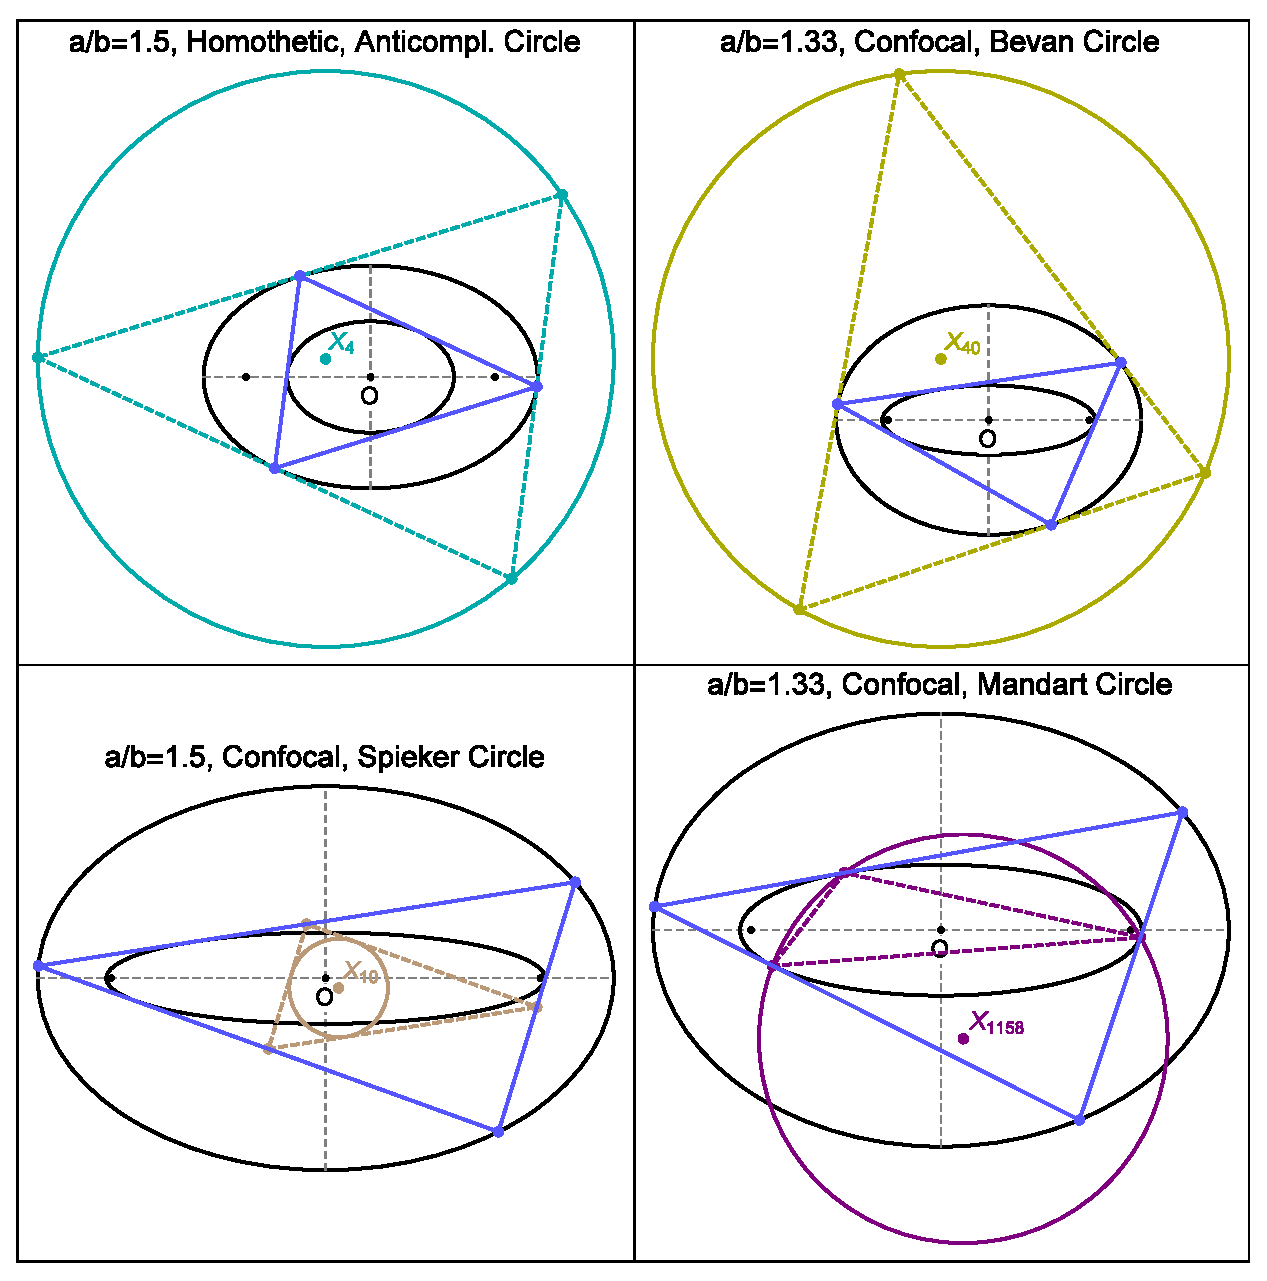
\includegraphics[width=.8\textwidth]{pics/0160_four_new_constant_power_circles.eps}
 \caption{Four additional circles (Anticomplementary, Bevan, Spieker, Mandart) with respect to which the power of the center is invariant, for the particular families indicated (homothetic, and thrice confocal, respectively). See these in motion at: \href{https://bit.ly/3qiTsgY}{\texttt{bit.ly/3qiTsgY}}, \href{https://bit.ly/3jPVvqf}{\texttt{bit.ly/3jPVvqf}}, \href{https://bit.ly/3bhOVFp}{\texttt{bit.ly/3bhOVFp}}, \href{https://bit.ly/3poGBbW}{\texttt{bit.ly/3poGBbW}}, respectively.}
 \label{fig:four-more}
\end{figure}

Additional circles and families show on Table~\ref{tab:addtl-circles} have been detected experimentally, with respect to which the center has constant power. We challenge the reader to derive them.

\begin{table}
\begin{tabular}{|l|l|l|l|}
\hline
Family & Triangle & Circle & Animation \\
\hline
Confocal & Extouch & Euler's & \href{https://bit.ly/3phwBkz}{\texttt{bit.ly/3phwBkz}} \\
Incircle & Intouch & Euler's & \href{https://bit.ly/2ZapHD0}{\texttt{bit.ly/2ZapHD0}} \\
Homothetic & Medial & Euler's & \href{https://bit.ly/3rTNQdc}{\texttt{bit.ly/3rTNQdc}} \\
Circumcircle & Euler's$^\ddagger$ & Euler's & \href{https://bit.ly/3qjytdY}{\texttt{bit.ly/3qjytdY}} \\
Dual$^\dagger$ & Euler's & Euler's & \href{https://bit.ly/2Nlx7AS}{\texttt{bit.ly/2Nlx7AS}}\\
Dual & Anticompl. & Circumc. & \href{https://bit.ly/3ai7BWg}{\texttt{bit.ly/3ai7BWg}}\\
Circumcircle & Orthic & Incircle & \href{https://bit.ly/3qhjhy0}{\texttt{bit.ly/3qhjhy0}} \\
\hline
\end{tabular}
\caption{Experimentally, the power of the center wrt certain additional family-circle combinations is also invariant. $^\ddagger$Euler's Triangle \cite{mw} has vertices at the midpoints of lines from the orthocenter $X_4$ to the vertices (they lie on Euler's circle).}
\label{tab:addtl-circles}
\end{table}

All of the examples in this section can be viewed in motion in \href{https://bit.ly/37dr1JJ}{bit.ly/37dr1JJ}.